\documentclass[]{article}
\usepackage{amssymb,amsmath}
\usepackage{ifxetex,ifluatex}
\usepackage[english]{babel}
\ifxetex
  \usepackage{fontspec,xltxtra,xunicode}
  \defaultfontfeatures{Mapping=tex-text,Scale=MatchLowercase}
\else
  \ifluatex
    \usepackage{fontspec}
    \defaultfontfeatures{Mapping=tex-text,Scale=MatchLowercase}
  \else
    \usepackage[utf8]{inputenc}
  \fi
\fi
\usepackage{graphicx}
% We will generate all images so they have a width \maxwidth. This means
% that they will get their normal width if they fit onto the page, but
% are scaled down if they would overflow the margins.
\makeatletter
\def\maxwidth{\ifdim\Gin@nat@width>\linewidth\linewidth
\else\Gin@nat@width\fi}
\makeatother
\let\Oldincludegraphics\includegraphics
\renewcommand{\includegraphics}[1]{\Oldincludegraphics[width=\maxwidth]{#1}}
\ifxetex
  \usepackage[setpagesize=false, % page size defined by xetex
              unicode=false, % unicode breaks when used with xetex
              xetex,
              colorlinks=true,
              linkcolor=black]{hyperref}
\else
  \usepackage[unicode=true,
              colorlinks=true,
              linkcolor=black]{hyperref}
\fi
\hypersetup{breaklinks=true, pdfborder={0 0 0}}
\setlength{\parindent}{0pt}
\setlength{\parskip}{6pt plus 2pt minus 1pt}
\setlength{\emergencystretch}{3em}  % prevent overfull lines
\setcounter{secnumdepth}{0}

\begin{document}

\begin{titlepage}
\centering \parindent=0pt
\newcommand{\HRule}{\rule{\textwidth}{1mm}}
\vspace*{\stretch{1}} \HRule\\[1cm]\Huge\bfseries
Simple Eye Tracker\\[0.7cm]
\large SIGB Assignment 1\\[1cm]
\HRule\\[4cm]  
\large by 
\\Morten Roed Frederiksen (mrof@itu.dk),  
\\Sigurt Dinesen (sidi@itu.dk),
\\Christoffer Stougaard Pedersen (cstp@itu.dk)\\ 
\vspace*{\stretch{2}} \normalsize %
\begin{flushleft}
IT-University of Copenhagen \\
SIGB, F2013\\
Dan Witzner Hansen \& Diako Mardanbeigi \\
\today \end{flushleft}
\end{titlepage}

\tableofcontents

\section{Introduction}

This is the first mandatory assignment for the course SIGB F2013. In
this assignment we'll implement a simple gaze tracker. This will be done
in the programming language python with help from the opencv and numpy
libraries.

This report is an attempt to document what has been done to make this
gaze tracker.

The basic structure for each section will be a short introduction of the
goal of the section, followed by the theory behind our approach ending
with a description of our actual implementation with visual aids used
for documentation. Additionally we will accompany the report with
captured videos demonstrating the usage of the eye tracker

\begin{figure}[htbp]
\centering
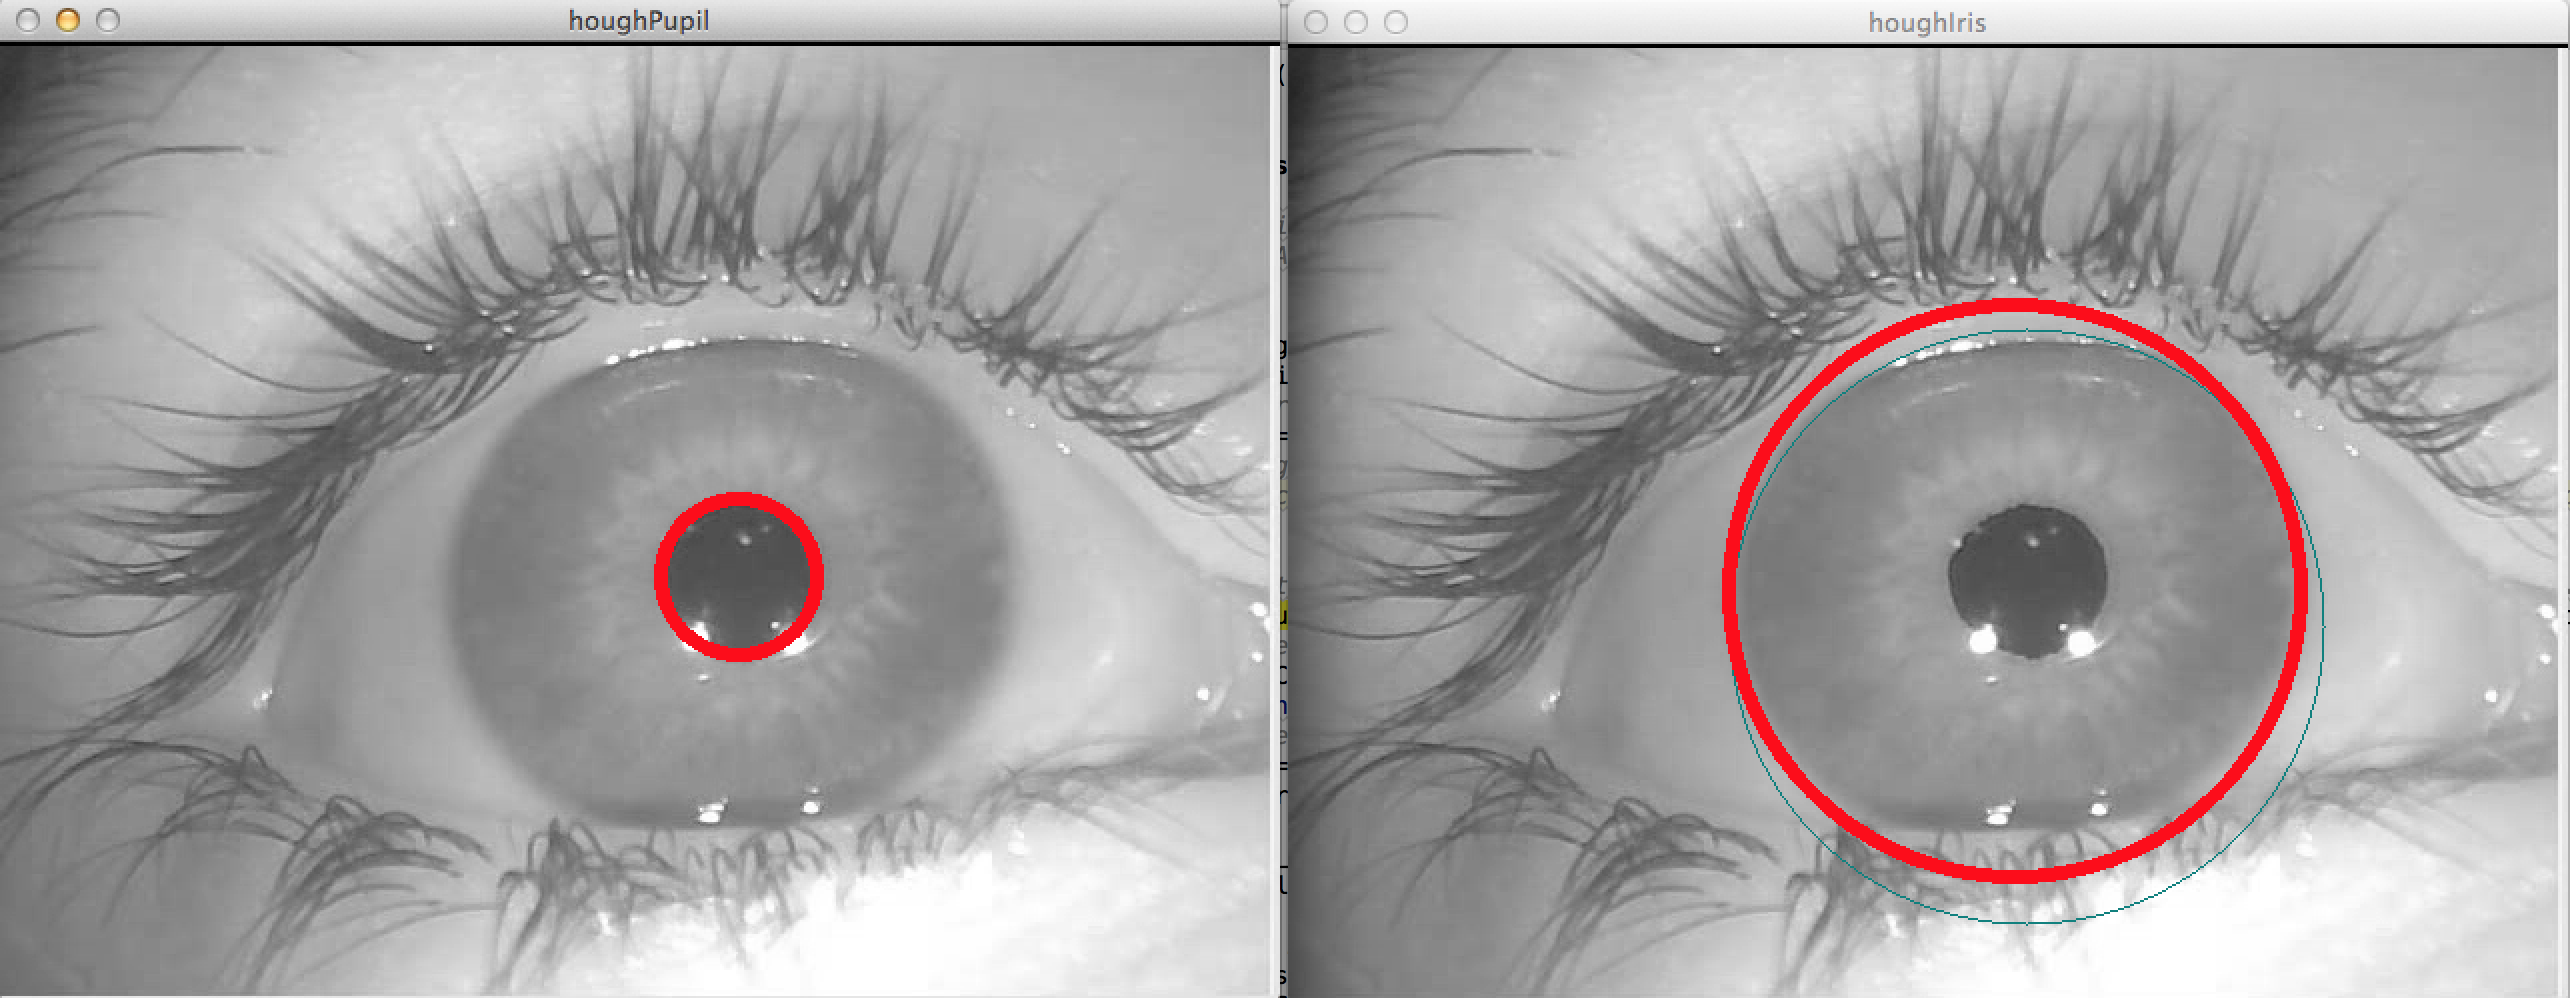
\includegraphics{pics/houghtransform.png}
\caption{Eye located with hough}
\end{figure}

\section{Pupil detection}

\subsection{Overall rationale and theory}

The eye consists of several distinct features such as pupil, iris,
limbus and sclera. Furthermore several features are present in images as
result of the light conditions when a picture is taken. The position of
these can aid in correctly determining the gaze. Detecting these
features is therefore a good starting for a gaze tracker implementation,
but it poses some challanges in correctly identifying each component,
and filtering away noise.

Of these features one of the easiest to recognize is the pupil, as it is
the darkest part of the eye. Furthermore it's good starting point, as it
is surrounded by the other eye components. The challenges/noise in
locating the pupil is mostly due to glints/reflections of light, but
these also aids in locating the pupil because we know that the pupil
will reflect light in a certain way.

As mentioned, the pupil is the darkest part of the eye. Furthermore a
pupil will reflect two ``glints'' of light. A good way to find the pupil
is to find an intensity value which can seperate it from the background.
This is called thresholding, and will be explained in the following
sections. Thesholding can be applied to both find pupil candidates as
well as glints used for more robustly picking the best pupil candidate.
When thresholding has been performed we will analyse certain features of
the BLOBs in the image to see which are good candidates for pupil and
glints. To aid in selected a proper threshold we will use a form of
pixel clasification to automatically set a threshold. This method will
be described last in this section.

\subsection{Thresholding}

Thresholding is a form of point processing used for seperating areas of
an image based on intensity in these areas. The desired end result of
this method is a binary image with the foreground (object) in one color
and the background (everything else) in a different color. This is
usually black and white respectively. This will effectively seperate the
foreground from the background for us, leaving us with only the
contours. In that sense we loose information and granularity in the
image, but since we're only interested in position we haven't lost
anything important.

\subsubsection{Theory}

As with all point processing methods the basic theory behind
thresholding is applying a calculation to every pixel in the image,
effectively changing the value of that pixel. We know that the end
result is a binary image, following this, each pixel will be transformed
into one of two values. We've so far operated on byte images so the max
value is 255 and the min value is of course 0. For clarity we will
assign each pixel either the min or the max value. Thus thresholding can
be expressed as the following with T being the assigned Threshold value
and f being the function applied to each pixel:

if f$(x,y) \leq T \quad then \, g$(x,y) = 0 \quad and \quad if
f$(x,y) < T \quad then \, g$(x,y) = 255

Performing these operations will leave us with an image where only
certain BLOBs are visible. We can then analyse the properties of these
BLOBs to find which one is most likely to be a pupil, and which are most
likely to be glints. Namely we will look at the area and the circularity
of blobs. Area is simply a count of all pixels in the blob.

Finding the circularity is a bit more complex. Used here is ``Heywoods
circularity factor'' which is derived from the perimeter and area of the
BLOB. Perimeter is the count of pixels on the rim of the contour. A
``cheaper'' approximation can be found by taking the perimeter of the
bounding box of a BLOB. The bounding box can be found simply by finding
the lowest and highest values of x and y respectively within a BLOB.

Once we have the perimeter and the area heywoods method can be applied.
It's defined as follows:

$Circularity = \frac {perimeter} {2 * \sqrt{\pi * area}}$

The area and circularity will be used to identify the best candidates

\subsubsection{Our implementation}

The usefulness of thresholding relies on having a total binary image
with the foreground easily distinguishable from the background. The
foreground is the pupil. The pupil is a dark circle-like object
surrounded by a lighter circle (the iris). So we're looking for a
threshold value that is lower than the surrounding iris. In an ideal
world the pupil in it's entirety will have only one intensity
throughout, and the ideal threshold value will be that. However, the
world is rarely so black and white (literally) and this also isn't the
case here. Although the pupil is the darkest spot it's not completely
dark. So a threshold value of 1 would be far to low in most
circumstances. It also requires very specialized lighting conditions to
achive a pupil with the same intensity throughout, so there is no
``silver bullet'' threshold value which will perfectly cover the entire
pupil.

What we're looking for is a value that is close enough to every part of
the pupil and far enough away from every part of the iris. The way of
finding this perfect value is mostly trial and error in this stage.
Luckily we had a slider to play around with when searching for this
value. For the thresholding itself, a built in cv2 method was used.

\begin{verbatim}
val,binI =cv2.threshold(gray, thr, 255, cv2.THRESH_BINARY_INV)
\end{verbatim}
Where:

gray is our (grayscale) image

thr is our selected threshold value

255 is the maximum value

the last argument is a constant indicating that output is a binary image

We quickly saw that a good value for most of the sequences floats around
100. An example of this can be seen in figure \ref{goodthr}:

\begin{figure}[htbp]
\centering
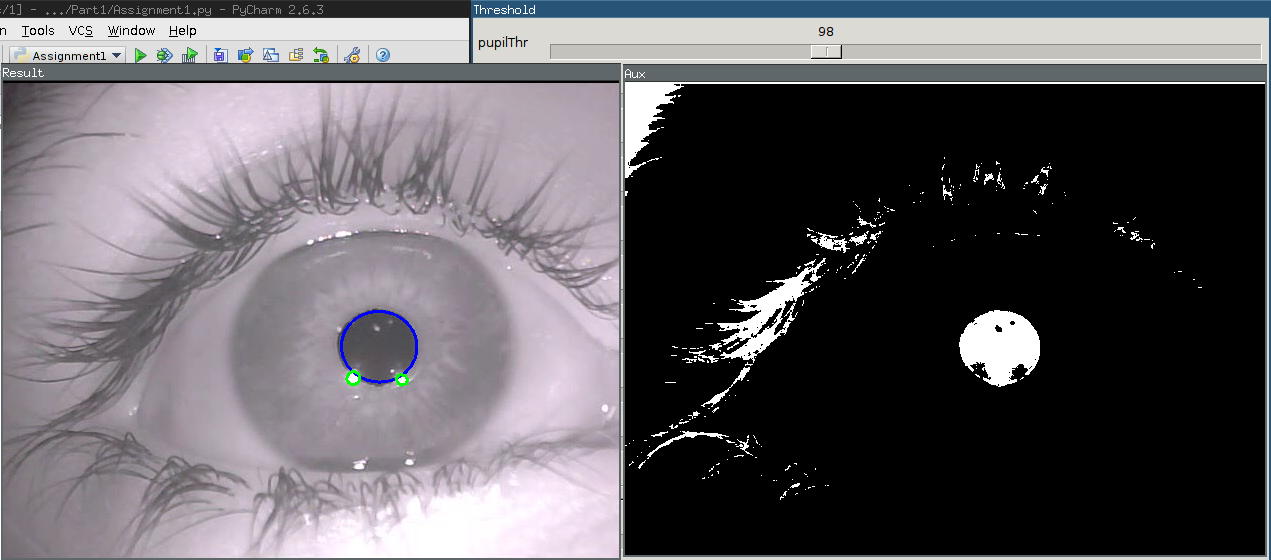
\includegraphics{pics/threshold_good.png}
\caption{Good threshold \label{goodthr}}
\end{figure}

This value is not robust in all cases, and too high or too low values
will yield to few or two many results respectively, seen in figures
\ref{lowthr} and \ref{highthr}

\begin{figure}[htbp]
\centering
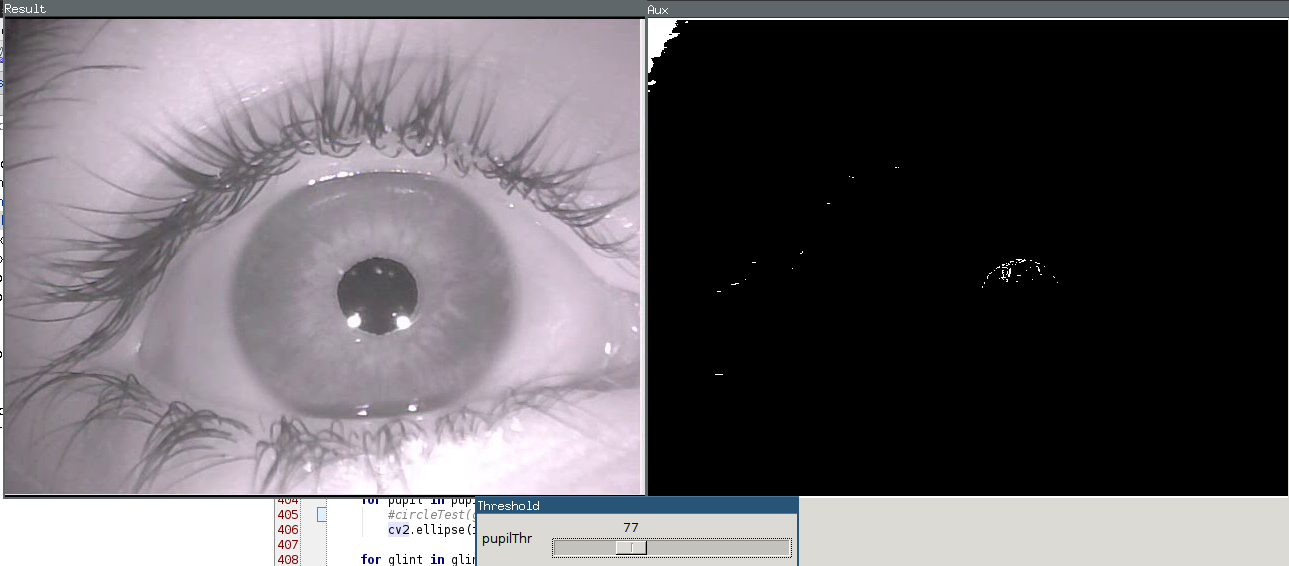
\includegraphics{pics/threshold_low.png}
\caption{Low threshold \label{lowthr}}
\end{figure}

\begin{figure}[htbp]
\centering
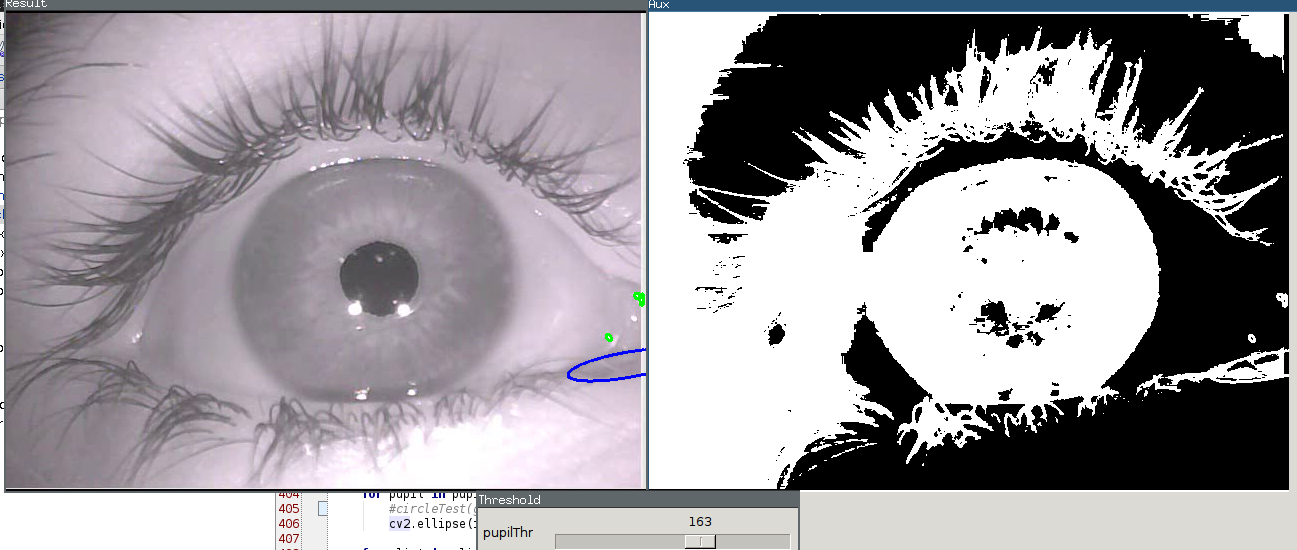
\includegraphics{pics/threshold_high.png}
\caption{High threshold \label{highthr}}
\end{figure}

Another aspect of this is that further analysis is needed on the
contours. So if a distorted figure is all we have it will be difficult
or impossible to correctly determine the nature of the contour. An
example of this false classification is seen in figure \ref{contourthr}

\begin{figure}[htbp]
\centering
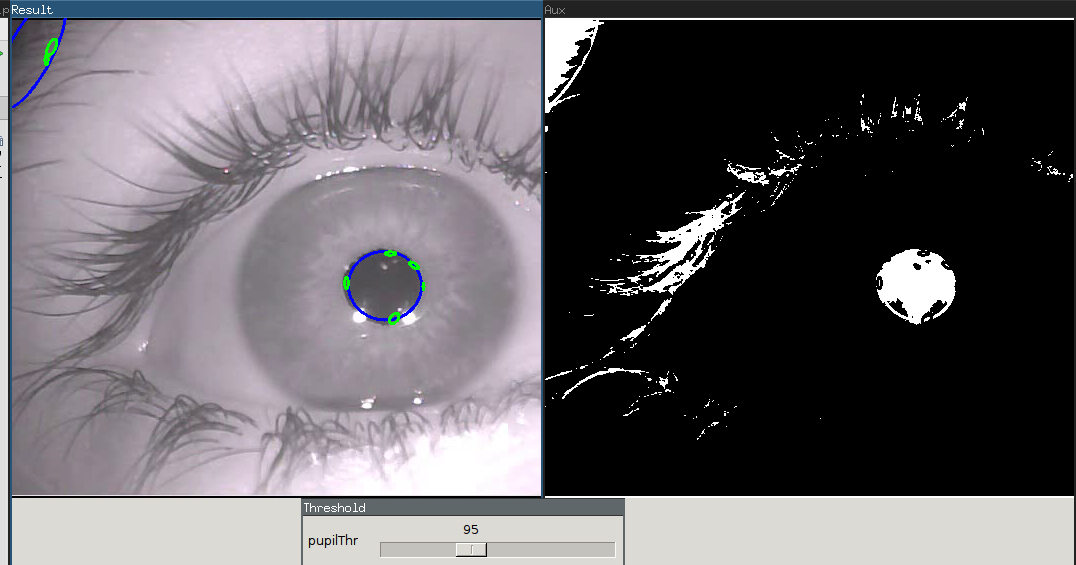
\includegraphics{pics/threshold_contours.png}
\caption{Contours found with threshold \label{contourthr}}
\end{figure}

In the happy path scenario analysis of the blobs will be performed as
described in the theory section above. First the area of the BLOB is
found:

This will be found using a cv2 methods. Presumably it's naively
implemented and has linear complexity, but this is speculation as we
don't have the implementation. Usage is as follows:

\begin{verbatim}
a = cv2.contourArea(con)
\end{verbatim}
Where con is a contour

Next the perimeters is found. Again opencv has an implementation for
this, given a closed contour:

\begin{verbatim}
p = cv2.arcLength(con, True)
\end{verbatim}
With these variables in hand the results can be filtered in a simple
imperative manner:

\begin{verbatim}
if(a==0 or a<minArea or a>maxArea):
    continue
p = cv2.arcLength(con, True)
m = p/(2.0*math.sqrt(math.pi * a))
if (m<1.7):
    if(len(con)>=5):
        ellips = cv2.fitEllipse(con)
        matches.append(ellips)
\end{verbatim}
The min and max area as well as the circularity value of 1.7 are found
through trial and error. The area parameters can be adjusted using
sliders as needed for each sequence. The constraints of the length of
the con is because we need 5 parameters for an ellipse

Last step is to redo this with the glints.

\begin{figure}[htbp]
\centering
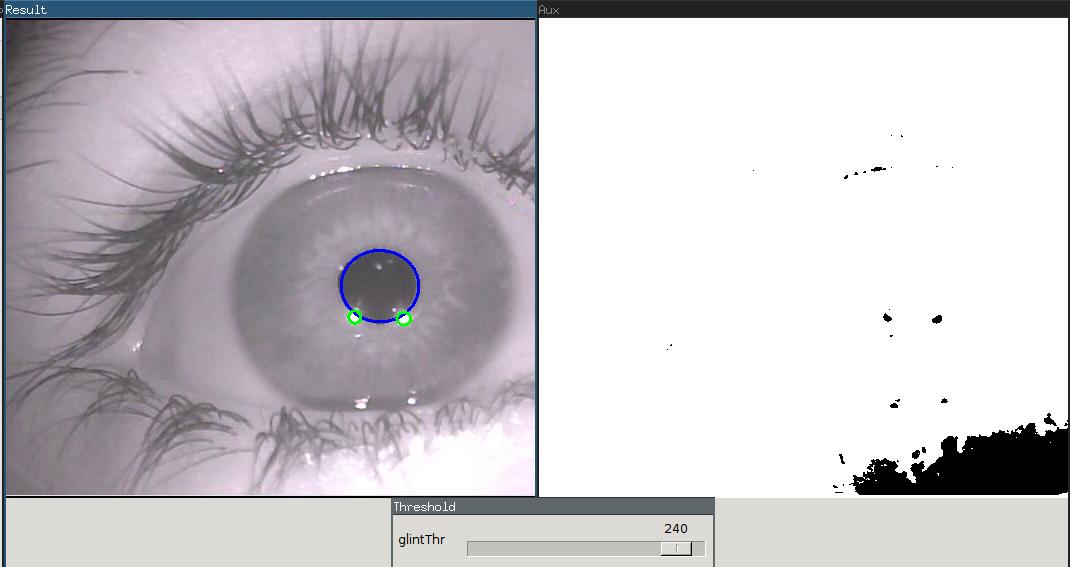
\includegraphics{pics/glintsthr.png}
\caption{Glints with threshold \label{glintsthr}}
\end{figure}

When we have the two glints of the pupil we can filter the data further
based on these newly found features. Out algorithm for this is very
straight forward and imperative:

\begin{verbatim}
for candA in glints:
    for candB in glints:
    #only accepting points with a certain distance to each other.
        if (Distance(candA[0],candB[0])> sliderVals['glintMinDist']
         and Distance(candA[0],candB[0]) < sliderVals['glintMaxDist']):
            glintList.append(candA)

#run through the remaining glints, keeping those that are 
#close to the pupil candidates.
for glintCand in glintList:
        for pupCand in pupils:
            if(Distance(glintCand[0],pupCand[0])>
            sliderVals['glint&pubMINDist'] and 
            Distance(glintCand[0],pupCand[0])<
            sliderVals['glint&pubMAXDist']):
                glintList1.append(glintCand)

#run through the pupil candidates keeping those that are close to 
#the fina glints list
for candP in pupils:
    for glintCand in glintList1:
        if(Distance(candP[0],glintCand[0])>
        sliderVals['glint&pubMINDist'] and 
        Distance(candP[0],glintCand[0])<
        sliderVals['glint&pubMAXDist']):
            pupilList.append(candP)

#sort out the pupils too far away from the found glints.
return (set(glintList1),set(pupilList))
\end{verbatim}
One critique of this approach could be that the pupil and glints depend
on each other ``both ways''. That is, we first filter the glint
candidates based on the pupil candidates and then the reverse is done.
However, the results seems to be fairly precise

\subsection{Pixel classification}

In this section it will be demonstrated how a form of machine learning
is applied to perform supervised classification in order to
semi-automatically set a correct thresholding value. Correct is defined
as a value which will allow us to perform the steps described in the
previous section

Clustering is the practice of grouping a set of elements into several
smaller groups of elements with similar features. It has a wide range of
applications within datamining and different types of analysis.
Obviously what will be demonstrated here is it's use within image
analysis. Clustering isn't a specific algorithm. Rather it's the task we
wish to perform in order to achieve our goal. In this assignment we've
used the k-means algorithm for this

K-means is a clustering algorithm which can group a number of
observations/data points into k number of clusters based on their
nearest mean value.

The properties of the k-means algorithm (k groups based on mean
intensity) combined with an existing knowledge of the properties of the
eye(the pupil is the darkest part) makes it possible to use k-means for
setting a threshold value automatically

\subsubsection{Theory}

The basic idea behind k-means clustering is to iteratively run through a
dataset assigning points in their correct cluster based on previously
selected values. Initially k points a selected and denoted as a center
for it's cluster, $c_1$ , \ldots{}, $c_k$ . These points can be selected
on random or based on some guessed distribution. On each run through the
dataset every points is examined. For each point the closest c is found,
and the point is marked as to belong to this cluster. Once all points
have been examined and placed in a cluster, the mean value of each
cluster is calculated as $c_ival$. Compare the mean value for the
cluster with the previously recorded value of $c_ival$. If it has
changed, another run through is performed. This continues until a
desired level of precision is achieved or amount of runs have taken
place

When we have done this we have k different threshold values to choose
from, given our knowledge of the pupil, we will choose the one with the
lowest mean value ($c_ival$).

\subsubsection{Our implementation}

There are a couple of possible caveats for this approach. Firstly there
is an element of uncertainty in exactly how the clusters will be
distributed. We need therefore to have a high enough k value to be sure
to get the right cluster. There is also some uncertainty about whether
the pupil always belongs to the darkest cluster. If for instance our
k-value is too high, and there exists a darker region in the image (dark
spot on the skin for instance) then the value of this cluster will be
chosen as a threshold value, and we might miss the pupil

Through trials it was found that 8 is a good value for k in the sense
that it often proved to segment the picture enough to allow the
intensity value of the pupil to exist in one of the clusters. The other
parameter is a constant that we apply so that the distance between the
points has less importance by dividing each point with this constant.
For this 15 was chosen as a good value.

The first step is performance optimization by resizing the image. This
saves a lot of computations:

\begin{verbatim}
smallI = cv2.resize(gray, reSize)
\end{verbatim}
where reSize is a 1x2 vector (30x30 was used)

When this is done we operate on column vectors

\begin{verbatim}
M,N = smallI.shape
X,Y = np.meshgrid(range(M),range(N))

z = smallI.flatten()
x = X.flatten()
y = Y.flatten()
O = len(x)
\end{verbatim}
From this we can create a ``feature'' matrix with values corresponding
to the intensity value of each pixel. Then the k-means algorithm is
applied to this feature-matrix to produce the centroids of each cluster.
The specifc k-means implementation comes from scipy. The same library
also provides a vector quantization which gives us the label for each
feature. Combining this we're left with a label image with intensities.
From these we pick the darkest and take that value as to mean the
intensity of the pupil. In reality this could probably be analysed
further to more robustly identify which cluster contains the pupil. For
instance we could analyse the original image and verify that there
exists an area with this intensity which looks sufficiently like a
pupil. If not, the second darkest area could be explored. This will
however further increase the computational complexity.

\begin{figure}[htbp]
\centering
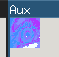
\includegraphics{pics/kmeans.png}
\caption{K-Means}
\end{figure}

\subsubsection{Usefulness of the k-Means algorithm}

K-Means seems very robust and definitely useful in applications like
this. A huge downside to this however is that it's computationally
expensive. Our implementation is at least. To overcome this we've used a
downsized image. As can be seen in figure \ref{kmeans}. This also makes
it very hard to visualize the method, as 30x30 pictures doesn't look to
great. If the downsizing isn't done, then the sequence can't really run.
One could argue that the lighting conditions of a picture rarely changes
on each frame. So doing k-means every time the frame is updated might be
overkill, and some calculations could be saved.


\end{document}
